\section{Graph Algorithm}

\subsection{Basic Stuff}

\subsubsection{Fundamental Concept}
The following is the basic concept of graph.
\begin{enumerate}
    \item A \textbf{graph} is a pair $G = (V,E)$.
    \item $V$ is set of vertices or nodes.
    \item $E$ is set of edges. An edge $e$ in $E$ is a pair of
        vertices $e = \{u,v\}$.
    \item If $G$ is undirected, $e$ is unordered, i.e. $e = uv = vu$.\\
        If $G$ is directed, $e$ is ordered, i.e. $e = u \rightarrow v$ or $(u,v)$.
    \item Graphs represent relations between pairs of objects.
\end{enumerate}

In this course, we mainly consider simple graphs,
no multi-edges and no self-loop.

\subsubsection{Concepts Used in this Note}
The following conclude the terminology and notations used
in this notes.

\begin{enumerate}
    \item The \textbf{degree} of $v$ is the number of adjacent edges.
    \item $n$ denotes $|v|$, $m$ denotes $|E|$.
    \item For undirected graph: $\displaystyle m \leq \binom{n}{2}$.
        For directed graph: $\displaystyle m \leq 2 \binom{n}{2}$.
    \item Sub-graph of $G=(V,E)$ is a graph $G^\prime = (V^\prime, E^\prime)$,
        s.t. $V^\prime \subseteq V$, $E^\prime \subseteq E$.
    \item A \textbf{walk} is a sequence $v_1\ldots v_l$,
        s.t. $v_i \in V$ and $v_iv_{i+1} \in E$.
    \item A \textbf{path} is a walk where $v_i$ distinct.
    \item A walk is close, if $v_i = V_k$.
    \item A cycle is a ``closed path''.
    \item Undirected graph connected if path between every pair $u,v \in V$.
    \item If not connected, a component is a maximal connect sub-graph.
    \item A \textbf{tree} is a connected ``acyclic'' graph.
    \item A \textbf{forest} is a graph where each component is a tree.
    \item A \textbf{Spanning Tree} of $G$ is a sub-graph that is a tree
        and contains all vertices of $G$.
    \item For directed graps: directed path/cycles.
    \item A graph is \textbf{Strongly Connected} if directed path
        from any vertex to another exists.
    \item Directed acyclic graph is called a \textbf{DAG}.
\end{enumerate}

\subsubsection{Graph Data Structure}
There are two widely used data structure of graph:
\begin{itemize}
    \item Adjacency Matrix: $|V| \times |V|$ matrix, where $A[i,j] = 1$
        if $(i,j) \in E$.
    \item Adjacency List: an array of length $|V|$, where
        every entry in the array stores a list of neighbors.
\end{itemize}

For example:
\begin{figure}[ht!]
    \caption{Example Graph}\label{example_graph}
    \centering
    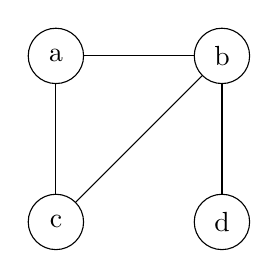
\begin{tikzpicture}
        \tikzstyle{every node}=[draw,circle,minimum size = 2em,node distance = 6em]
        \node (a) {a};
        \node [right of = a] (b) {b} edge(a);
        \node [below of = a] (c) {c} edge(a) edge(b);
        \node [below of = b] {d} edge(b);
    \end{tikzpicture}
\end{figure}

The adjacency matrix and adjacency list for \cref{example_graph} would be:
\begin{table}[ht!]
\begin{minipage}[b]{0.56\linewidth}
\centering
    \begin{tabular}{l|llll}
        & A & B & C & D \\ \hline
         A & 0  & 1  & 1  & 0  \\
         B & 1  & 0  & 1  & 1  \\
         C & 1  & 1  & 0  & 0  \\
         D & 0  & 1  & 0  & 0  \\
    \end{tabular}
    \caption{Adjacency Matrix}
    \label{table:student}
\end{minipage}\hfill
\begin{minipage}[b]{0.4\linewidth}
\centering
\begin{tikzpicture}
    \matrix (M) [matrix of nodes,
                column sep=-\pgflinewidth,
                row sep=0pt,
                nodes in empty cells,
                nodes={draw,fill=gray!20,minimum width=.5cm,outer sep=0pt,minimum height=.7cm,anchor=center},
                column 1/.style={minimum height=.8cm, minimum width=2em}]{
        a &[8mm] b & \mbox{} &[4mm] c & /       \\
        b & a      & \mbox{} & c      & \mbox{}  & [4mm]d    & /  \\
        c & a      & \mbox{} & b      & /         \\
        d & b      & \mbox{} & /      & \mbox{}  \\
    };
    \foreach \i in {1,2,3,4}{
        \path (M-\i-1) [late options={label=left:\i}];
        \draw[->] (M-\i-1.east)--(M-\i-2.west);
        \draw[->] (M-\i-3.center)--(M-\i-4.west);
    }
    \draw[->] (M-2-5.center)--(M-2-6.west);
\end{tikzpicture}
\captionof{figure}{Adjacency List}
\label{fig:image}
\end{minipage}
\end{table}

The running time for these two data structures are shown in
\cref{table:running_time_of_amaj}.

\begin{table}[H]
    \caption{Running Time Analysis for Adjacency Matrix and Adjacency List}
    \label{table:running_time_of_amaj}
    \centering
    \begin{tabular}{l|c|c}
        \hline
        Time & Adjacency Matrix & Adjacency List \\\hline
        visit neighbor & \bigO{1} & \bigO{1}\\
        visit all neighbors & \bigO{n} & \bigO{degree(v)} \\
        test if $uv \in E$ & \bigO{1} & \tikzmark{runanaadaj1}{\bigO{degree(v)}}\\
        add/delete edge & \bigO{1} & \tikzmark{runanaadaj2}{\bigO{n}}\\
        size & \bigO{mn} & \bigO{m+n}
    \end{tabular}
    \begin{tikzpicture}[remember picture,overlay,node distance = 1cm]
        \node[below right = 4em and 1em of runanaadaj1] (notes) {\bigO{1} with hashing.};
        \draw[->,thick] (runanaadaj1.east) to [in=90,out=0] (notes.north);
        \draw[->,thick] (runanaadaj2.east) to [in=90,out=0] (notes.north);
    \end{tikzpicture}
\end{table}

